%Part of/Parte di https://github.com/f-dinucci/appuntiMeccanicaFluidi/
%License/Licenza Creative Commons Attribution-ShareAlike 4.0 International (CC BY-SA 4.0) - attribution/attribuzione Francesco Di Nucci
%See also/Vedere anche https://creativecommons.org/licenses/by-sa/4.0/ and/e https://creativecommons.org/licenses/by-sa/4.0/legalcode
%
\section{Strato limite}

%SUBSECTION
\subsection{Strato limite}
Si è visto che in un sottile strato vicino alla parete i comportamenti delle equazioni di Eulero e Navier-Stokes differiscono, occorre quantificare questo fenomeno.
 %
	\begin{figure}[ht]
		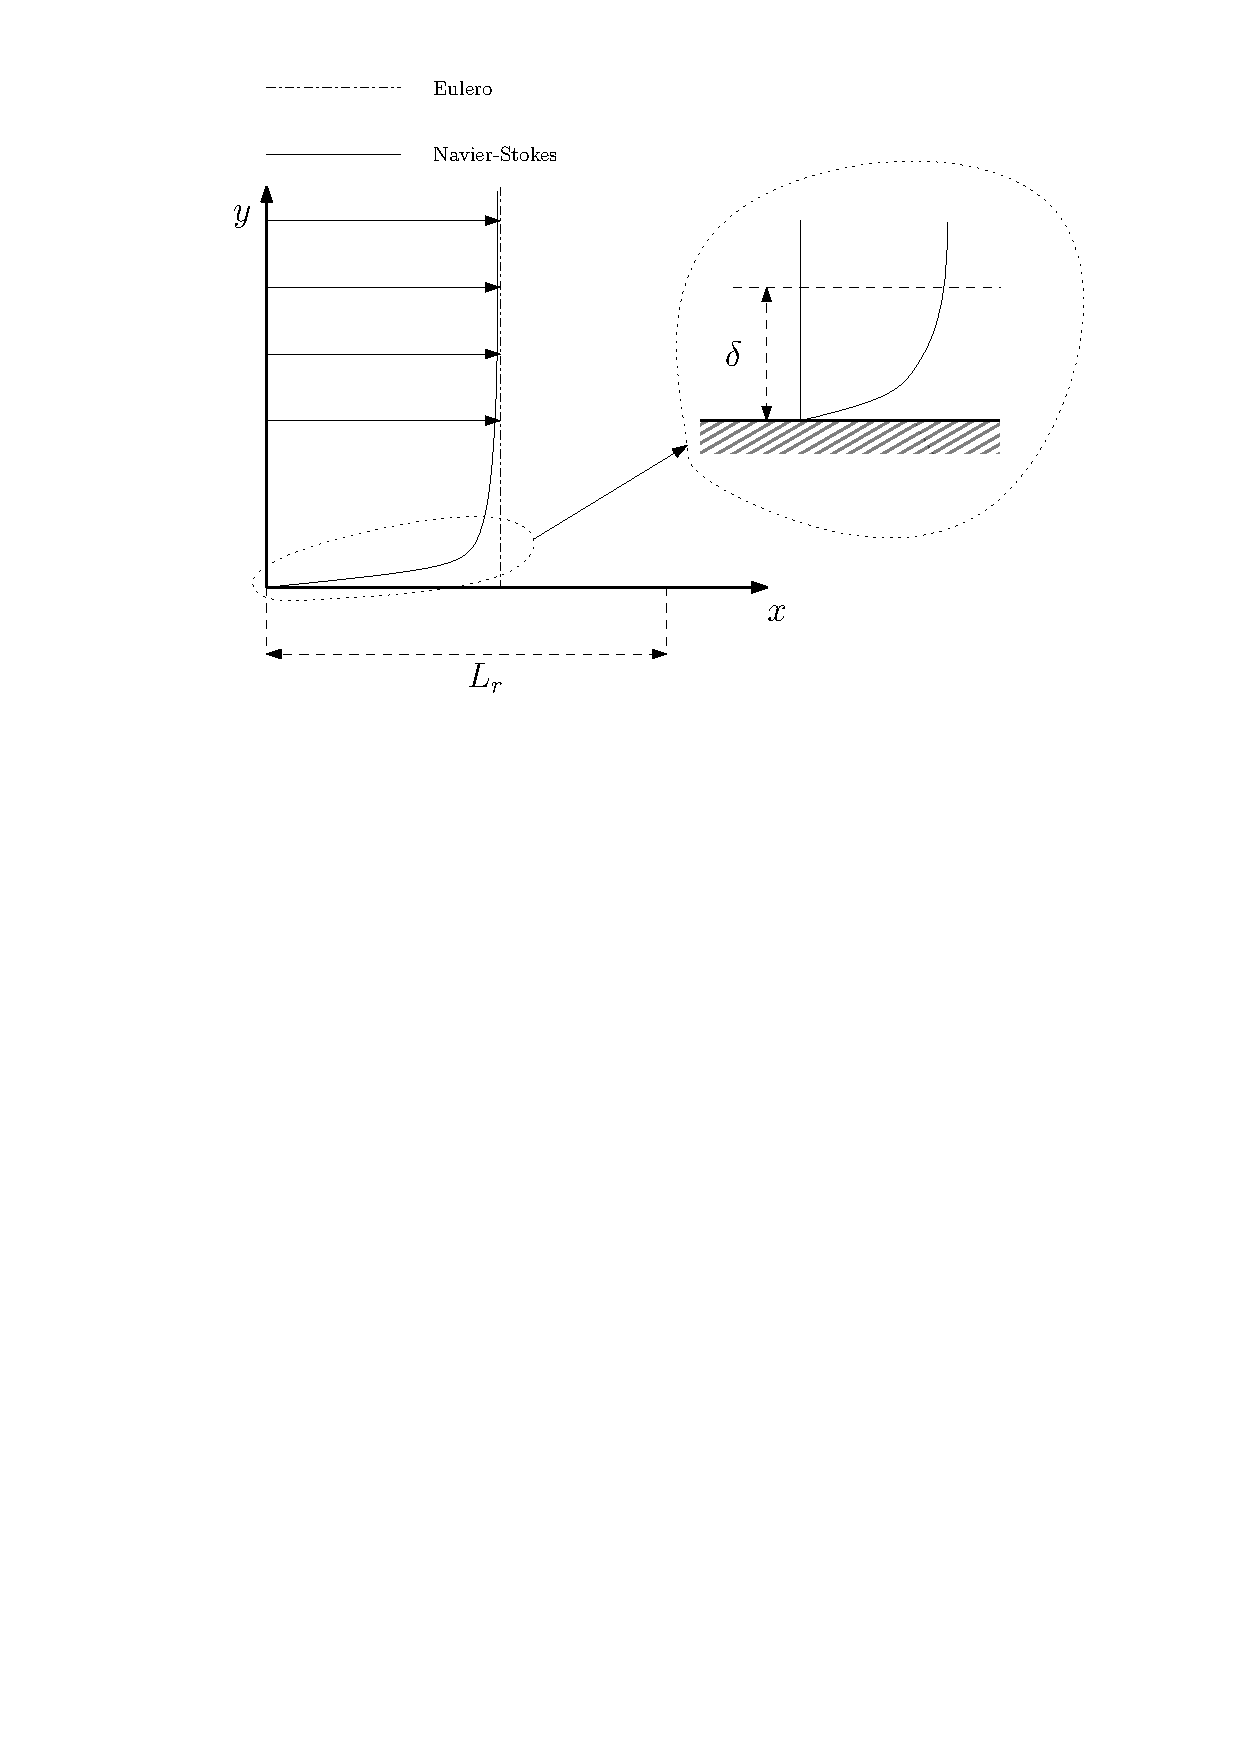
\includegraphics[scale=0.85]{./7.4 Strato limite/7.4-1}
		\centering
		\caption{Strato limite}
	\end{figure}
%

Nel caso bidimensionale, stazionario, per fluido non viscoso si ha che:
%
	\begin{equation*}
		\begin{gathered}
			u_x + v_y = 0\\
			u u_x + v u_y + \frac{1}{\rho} p_x = \nu (u_{xx} + u_{yy})
		\end{gathered}
	\end{equation*}
%
Nel caso turbolento per via del numero di Reynolds alto si trascura il secondo termine e si arriva alle equazioni di Eulero.
Nello strato limite però la derivata $u_{yy}$ è grande e compensa il numero di Reynolds, quel termine quindi non è più trascurabile.
Affinché ciò accada, come ordini di grandezza si vuole che:
%
	\begin{equation*}
		\begin{gathered}
			\nu u_{yy} \sim \frac{U_r}{\delta^2}\\
			\nu \sim \frac{U^2_r}{L_r}
		\end{gathered}
	\end{equation*}
%
Si parte dall'equazione in forma dimensionale:
%
	\begin{equation*}
		u u_x + v u_y + \frac{1}{\rho} p_x = \nu (u_{xx} + u_{yy})
	\end{equation*}
%
Per quanto visto prima come ordini di grandezza si ha che:
%
	\begin{equation*}
		\begin{gathered}
			\left( \frac{\delta}{L_r} \right) \sim \frac{\nu}{v_r L_r} = \frac{1}{R_e}\\
			\frac{\delta}{L_r} = \frac{1}{\sqrt{R_e}}
		\end{gathered}
	\end{equation*}
%
Quindi adimensionalizzando:
%
	\begin{equation*}
		\begin{gathered}
			u_x + v_y = 0\\
			u u_x + v u_y + p_x = \frac{1}{R_e} (u_{xx} + u_{yy})\\
			u v_x + v v_y + p_y = \frac{1}{R_e} (v_{xx} + v_{yy})
		\end{gathered}
	\end{equation*}
%
Si effettua poi un cambiamento di variabili:
%
	\begin{equation*}
		\begin{gathered}
			y = \epsilon Y\\
			\epsilon = \frac{\delta}{L_r}\\
			v = \epsilon V
		\end{gathered}
	\end{equation*}
%
Quindi si trova che:
%
	\begin{equation*}
		\begin{gathered}
			y = \frac{y^d}{L_r}\\
			\epsilon = \frac{\delta}{L_r}\\
			\text{allora}\\
			Y = \frac{y^d}{\delta}
		\end{gathered}
	\end{equation*}
%
Le equazioni adimensionali diventano allora:
%
	\begin{equation*}
		\begin{gathered}
			u_x + V_Y = 0\\
			u u_x + V u_Y + p_x = \frac{1}{R_e} u_{xx} + \frac{1}{R_e \epsilon^2} u_{YY}\\
			\epsilon u V_x + \epsilon V V_Y + \frac{1}{\epsilon} p_Y = \frac{\epsilon}{R_e} V_{xx} + \frac{1}{R_e \epsilon} V_{YY}
		\end{gathered}
	\end{equation*}
%
Scegliendo:
%
	\begin{equation*}
	 	\epsilon = \frac{1}{\sqrt{R_e}}
	\end{equation*}
%
Si ottiene che:
%
	\begin{equation*}
	 	\frac{1}{R_e \epsilon^2} = 1 \quad \frac{\epsilon}{R_e} = \epsilon^3
	\end{equation*}
%

Al limite per $R_e \rightarrow \infty$ e $\epsilon \rightarrow 0$ si arriva alle \textbf{equazioni dello strato limite di Prandtl}:
%
	\begin{equation*}
		\begin{gathered}
			u_x + V_Y = 0\\
			u u_x + V u_Y + p_x = u_{YY}\\
			p_Y = 0
		\end{gathered}
	\end{equation*}
%
In $y$ c'è una derivata seconda, sulla $x$ invece si ha una equazione parabolica.
Si dimostra che le condizioni al contorno devono soddisfare un dominio a C:
 %
	\begin{figure}[ht]
		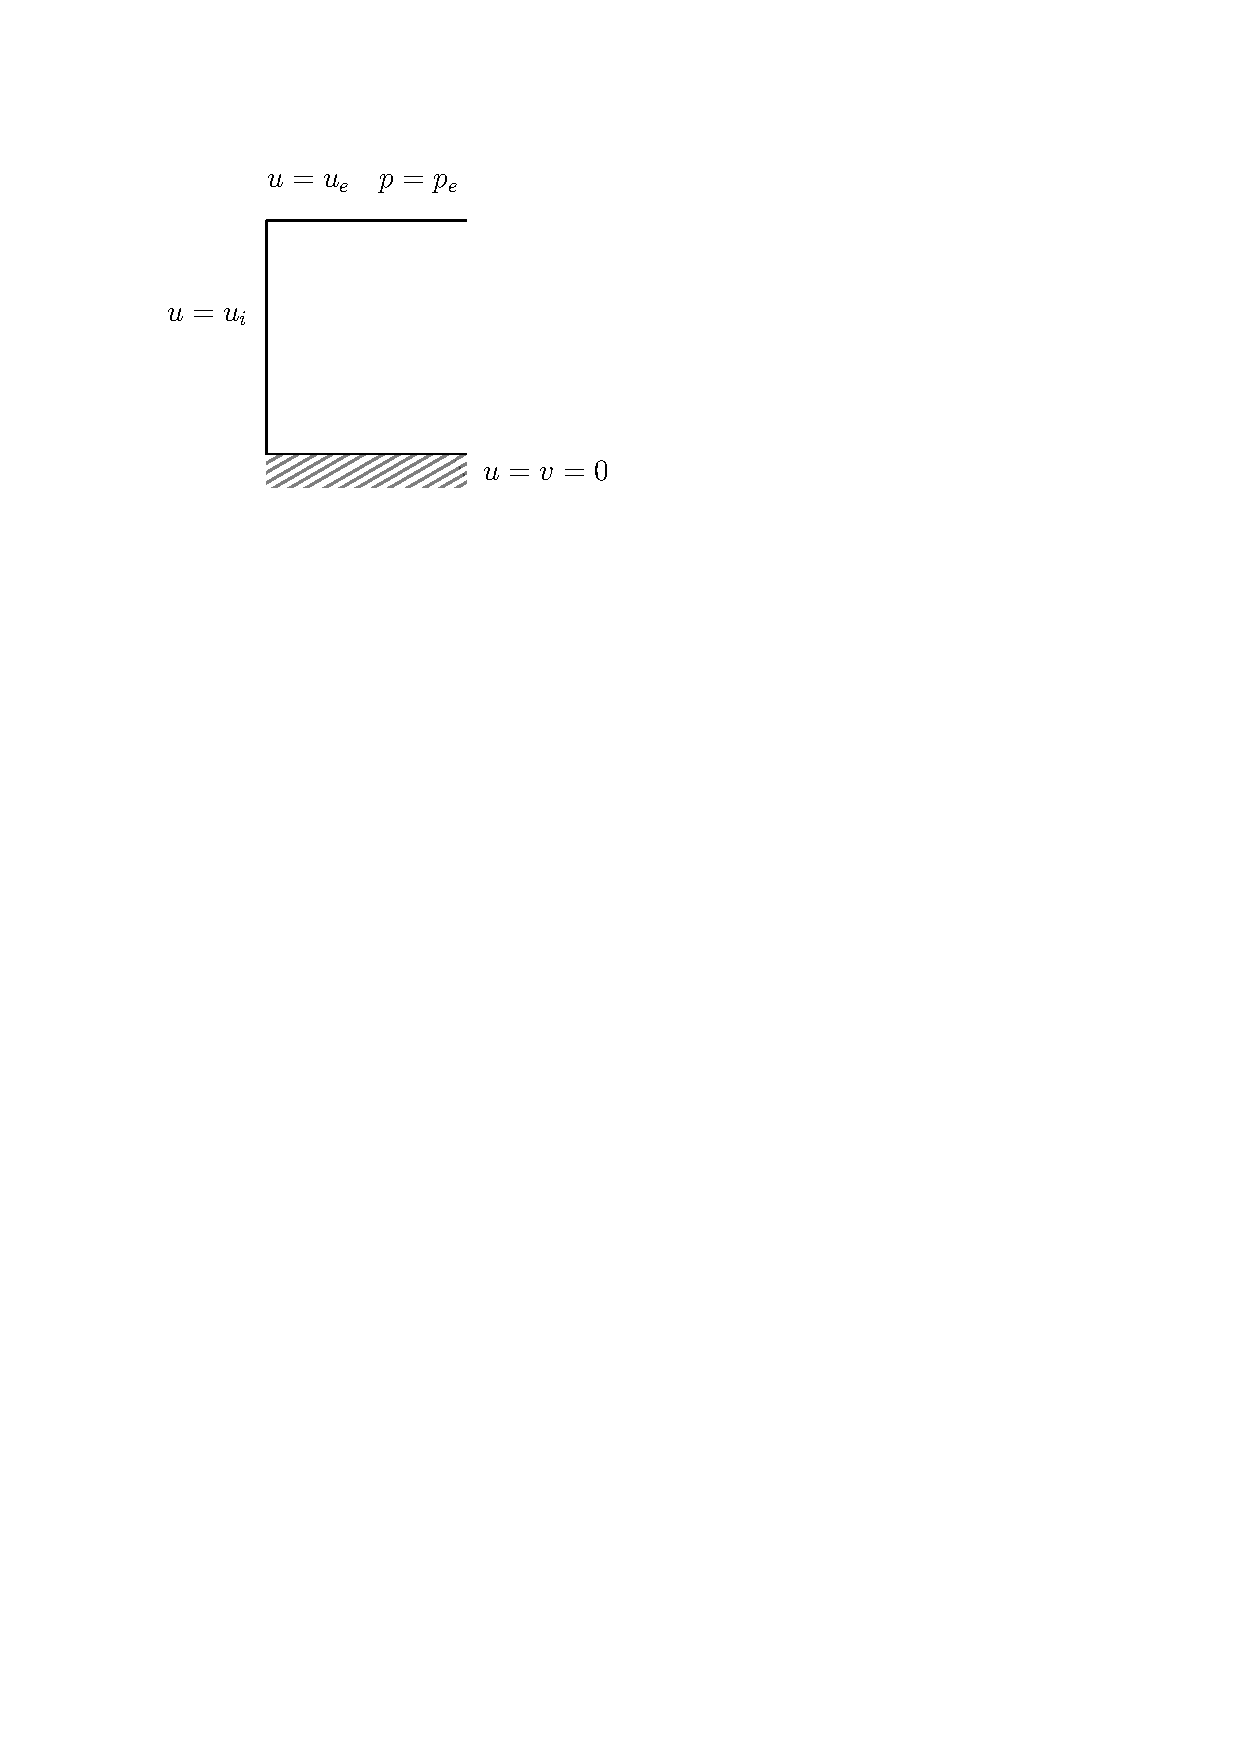
\includegraphics[scale=0.7]{./7.4 Strato limite/7.4-2}
		\centering
		\caption{Dominio a C}
	\end{figure}
%
Si possono fare delle semplificazioni e tenere conto che $p_e$ obbedisce alle equazioni di Eulero (e quindi alla legge di Bernoulli):
%
	\begin{equation*}
		\begin{gathered}
			p_Y = 0 \rightarrow p = p(x) = p_e\\
			p_e + \frac{1}{2} u^2_e = cost.
		\end{gathered}
	\end{equation*}
%
Derivando $p_{e,x} = - u_e u_{e,y}$, sostituendo si ottengono le equazioni di Prandtl senza la pressione:
%
	\begin{equation*}
		\begin{gathered}
			u_x + V_Y = 0\\
			u u_x + V u_Y = u_e u_{e,x} + u_{YY}
		\end{gathered}
	\end{equation*}
%
Al posto dell'equazione di continuità si introduce la funzione di corrente:
%
	\begin{equation*}
		\begin{gathered}
			\psi_Y = u\\
			\psi_x = - V\\
			\psi_Y \psi_{xY} - \psi_{x} \psi_{YY} = u_e u_{e,x} + \psi_{YYY}
		\end{gathered}
	\end{equation*}
%

%SUBSECTION
\subsection{Lastra piana ed equazione di Blasius} 
È possibile cercare una soluzione in casi particolari.
Dato che le equazioni dello strato limite valgono solamente in un sottilissimo strato a contatto con la parete, è indifferente trattare una lastra piana o curva, dato che a confronto il raggio di curvatura sarebbe molto grande (cambierebbe solamente l'espressione di $p_e$)

Se sceglie $u_e$ come riferimento, per il flusso su una lastra piana la condizione al contorno è $u_e = cost. = 1$.
Da questo le condizioni al contorno possono essere espresse come:
%
	\begin{equation*}
		\begin{gathered}
			Y = 0 \rightarrow \quad \psi = \psi_Y = 0\\
			Y \rightarrow \infty \quad \psi_Y = 1\\
			x = 0 \quad \psi_Y = 1
		\end{gathered}
	\end{equation*}
%
Si vede allora se esiste una soluzione simile/di similitudine.
Si ipotizza che:
%
	\begin{equation*}
		u = f \left( \frac{Y}{x^a} \right)
	\end{equation*}
%	
Si impone poi che:
%
	\begin{equation*}
		\begin{gathered}
			f(0) = f'(0) = 0\\
			f(\infty) = 1 
		\end{gathered}
	\end{equation*}
%
Quindi:
%
	\begin{equation*}
		\begin{gathered}
			\psi = x^a F \left( \frac{Y}{x^a} \right)\\
			F' = f
		\end{gathered}
	\end{equation*}
%
Si calcolano le derivate:
%
	\begin{equation*}
		\psi_Y = F' \quad \psi_{YY} = x^{-a} F'' \quad \psi_{YYY} = -x^{-2a} F'''
	\end{equation*}
%
E sostituendo
%
	\begin{equation*}
		\begin{gathered}
			\psi_x = a x^{a-1} F - a x^{-1} Y F'\\
			\psi_{xy} = \psi_{yx} = - a x^{-a-1} Y F''
		\end{gathered}
	\end{equation*}
%
Sostituendo nuovamente:
%
	\begin{equation*}
		\begin{gathered}
			\psi_{Y} \psi_{xY} - \psi_{x} \psi_{YY} = \psi_{YYY}\\
			F' (-a x^{-a-1} Y F'') - x^{-a} F'' (a x^{a-1} F - a x^{-1} y F') = x^{-2a} F'''
		\end{gathered}
	\end{equation*}
%			
E semplificando:
%
	\begin{equation*}
		\begin{gathered}		
			-a x^{-1} F F'' = x^{-2a} F''' \rightarrow a = \frac{1}{2}\\
			F''' + \frac{1}{2} F F'' = 0 \quad \textbf{Equazione di Blasius}
		\end{gathered}
	\end{equation*}
%
L'equazione di Blasius è una equazione ordinaria in una variabile.
Poi:
%
	\begin{equation*}
		\begin{gathered}
			F(0) = F'(0) = 0\\
			F'(\infty) = 1\\
			F(\eta)\\
			\text{dove}
			\eta = \frac{y}{x^{1/2}}
		\end{gathered}
	\end{equation*}
%
Non esiste una soluzione analitica di questa, ma è una funzione nota, si può quindi tracciarne un grafico e calcolarne i valori al computer:
 %
	\begin{figure}[ht]
		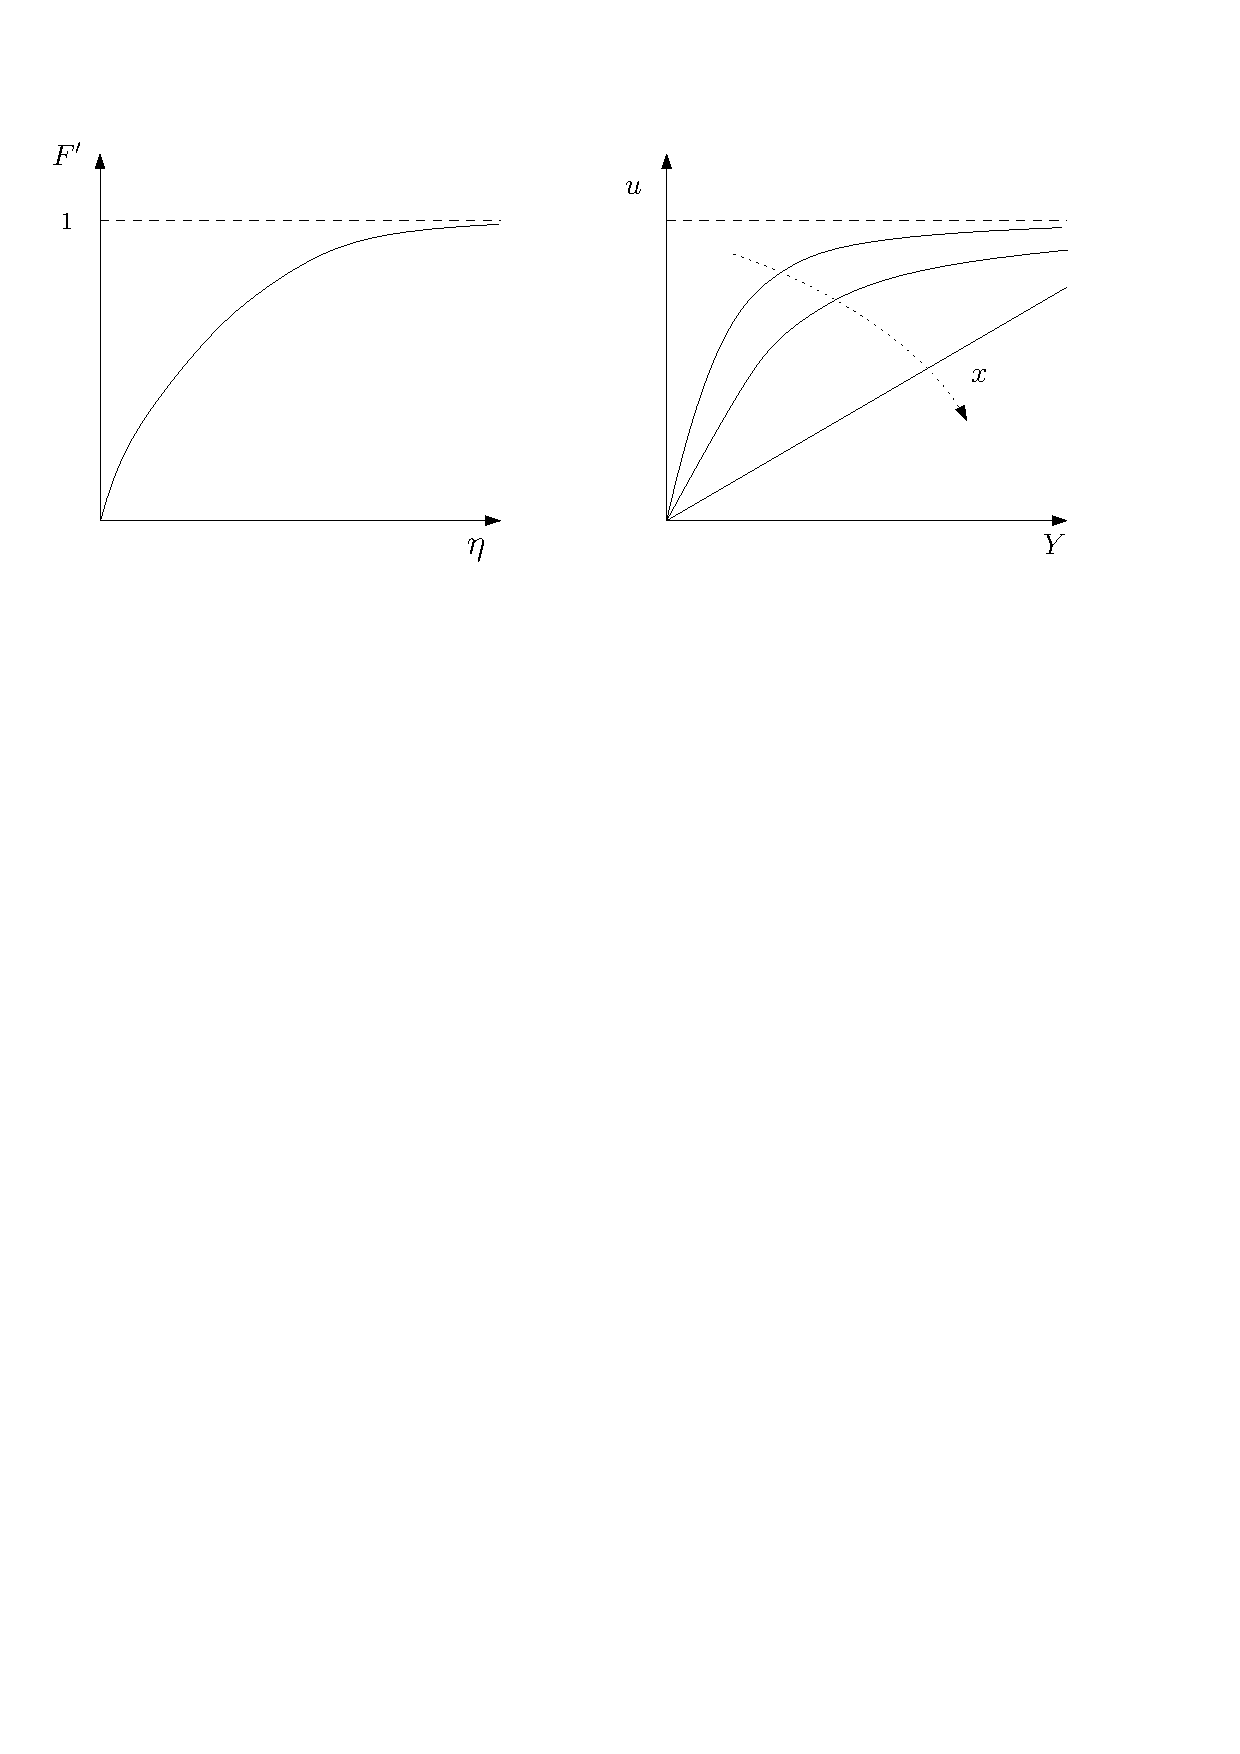
\includegraphics[scale=0.7]{./7.4 Strato limite/7.4-3}
		\centering
		\caption{Grafici in funzione di $\eta$ e $Y$}
	\end{figure}
%
Notare che lo spessore dello strato limite aumenta con la velocità.

%SUBSECTION
\subsection{Coefficiente d'attrito}
È noto che $F''(0) = 0.322\ldots$, occorre approfondire, serve per l'attrito a parete
Si fa percorso inverso a partire dallo sforzo:
%
	\begin{equation*}
		\begin{gathered}
			\tau^d = \mu \pdv{u^d}{y^d} = \mu \frac{U^r}{L^r} \pdv{u}{y} = \mu \frac{U^r}{L^r \epsilon} \pdv{u}{Y} = \frac{\mu U^r}{\epsilon L^r x^{1/2}} \pdv{u}{\eta} = \frac{\mu U^r}{\epsilon L^r x^{1/2}} F'' =\\
			= 0.332 \frac{\mu U^r}{\epsilon L_r x^{1/2}} = 0.332 \rho U^2_r \frac{1}{\epsilon R_e x^{1/2}} = 0.332 \rho U^2_r \frac{1}{R_e^{1/2} x^{1/2}}
		\end{gathered}
	\end{equation*}
%
Si introduce il coefficiente di attrito, sostanzialmente una $\tau$ adimensionale, definito come:
%
	\begin{equation*}
		\begin{gathered}
			C_f = \frac{\tau}{1/2 \rho U^2_r} = 0.664 R_e^{-1/2} x^{-1/2} = 0.664 R_{ex}^{-1/2}\\
			\text{dove} \quad R_{ex} = \frac{x^d U^r}{\nu}
		\end{gathered}
	\end{equation*}
%
Oppure si possono quindi semplificare tutte le grandezze adimensionali per arrivare ad una grandezza dimensionale:
%
	\begin{equation*}
		\begin{gathered}
			\tau^d = 0.332 \frac{\mu U^r}{\epsilon L^r x^{1/2}} = 0.332 \frac{\mu U^r}{ {\left( \frac{\nu}{U^r L^r} \right)}^{1/2} {\left( \frac{x^d}{L^r} \right)}^{1/2} L^r } = 0.332 \rho \nu^{1/2} {U^r}^{3/2} {x^d}^{-1/2}
		\end{gathered}
	\end{equation*}
%
È completamente dimensionale e non è costante, è una $f(x)$.

Per la forza sulla parete:
%
	\begin{equation*}
		F^d = \int_0^L \tau^d \dd{x^d} = 2 \vdot 0.332 \rho \nu^{1/2} {U^r}^{3/2} L^{1/2}
	\end{equation*}
%
 %
	\begin{figure}[ht]
		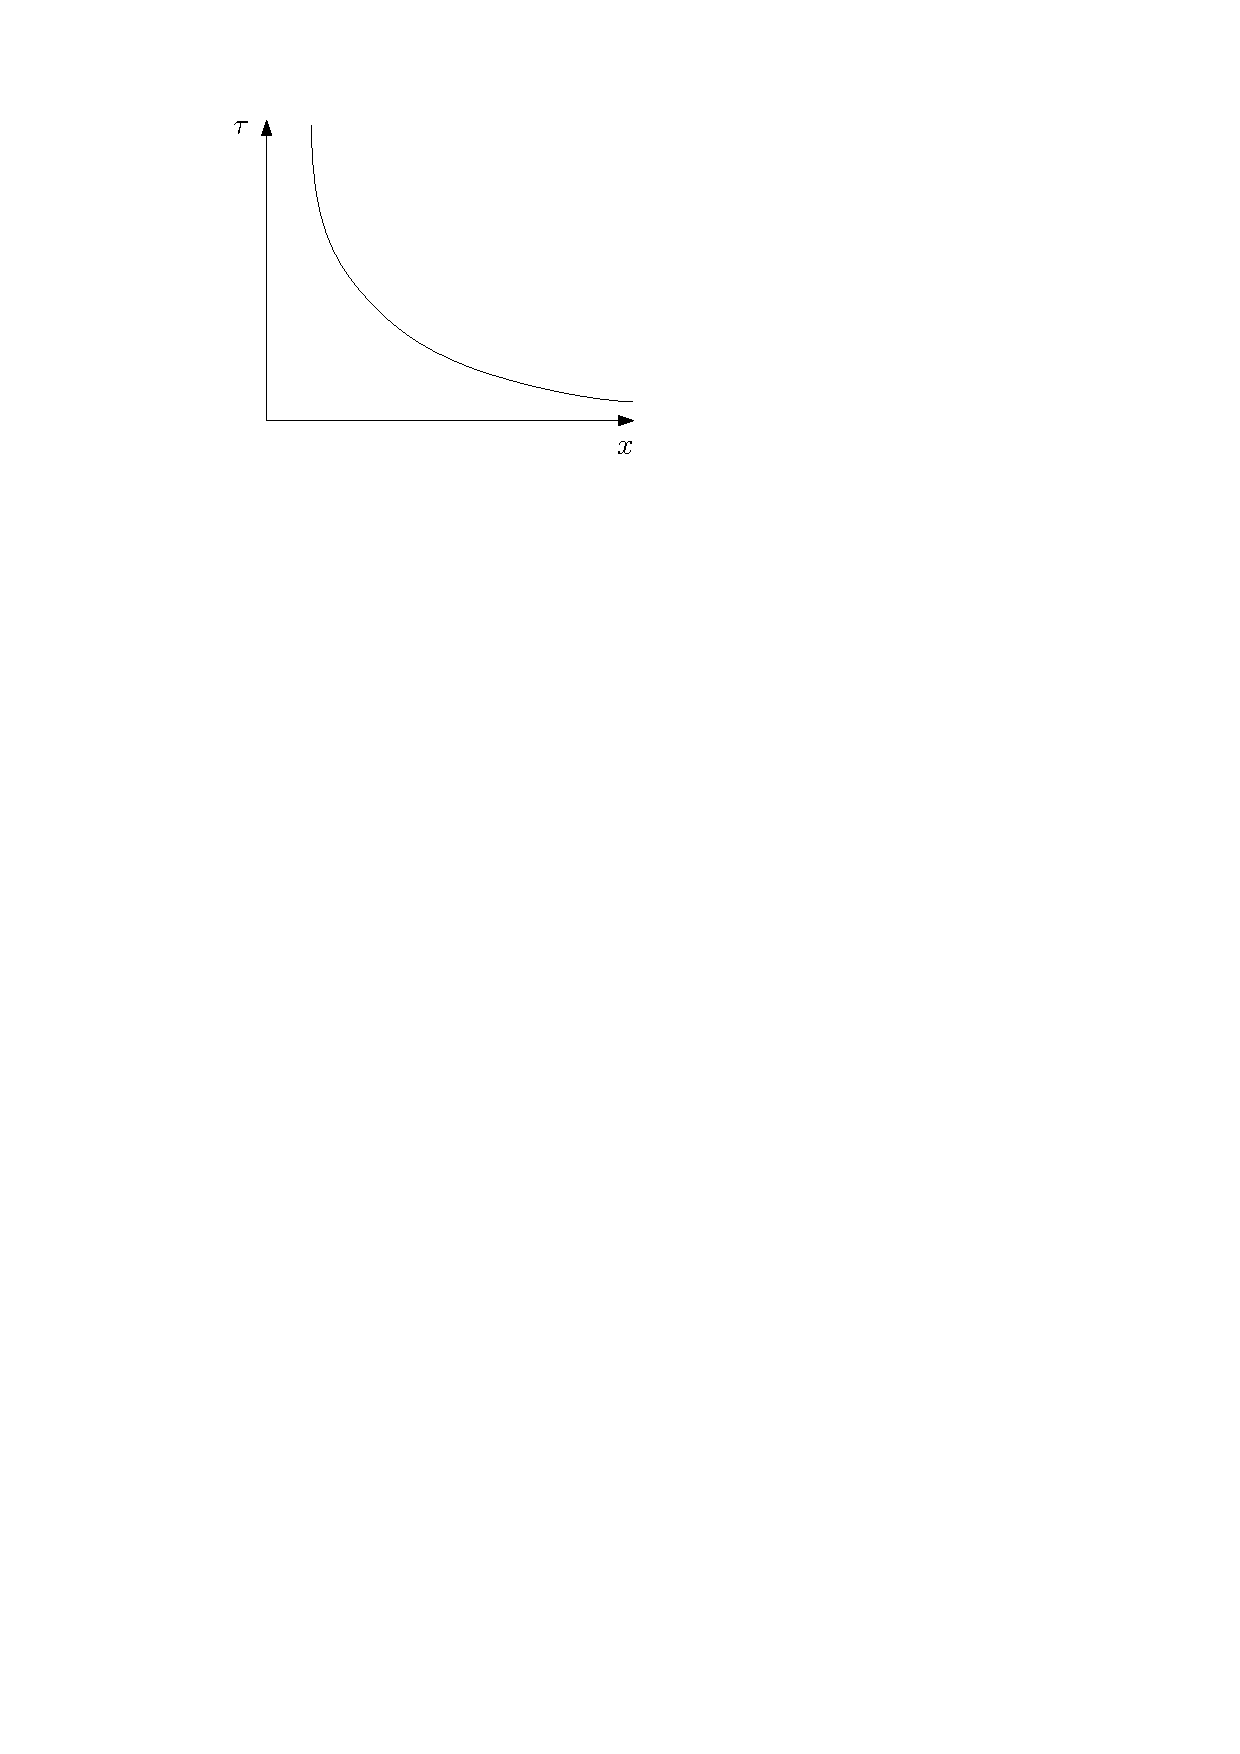
\includegraphics[scale=0.8]{./7.4 Strato limite/7.4-4}
		\centering
		\caption{Diagramma dello sforzo}
	\end{figure}
%

$x^{-1/2}$ dà una singolarità integrabile, all'inizio lo sforzo tende ad infinito ma la forza è comunque finita: all'attacco della parete non vale il modello di strato limite ma quello di Navier-Stokes, lo sforzo non va realmente ad infinito dato che il contributo del termine $\tau \rightarrow \infty$ è trascurabile.

%SUBSECTION
\subsection{Spessore dello strato limite}
$F(\eta)$ è una funzione continua, si prendono dei riferimenti, ad esempio si valuta dove la velocità è pari al 99\% di quella esterna:
 %
	\begin{figure}[ht]
		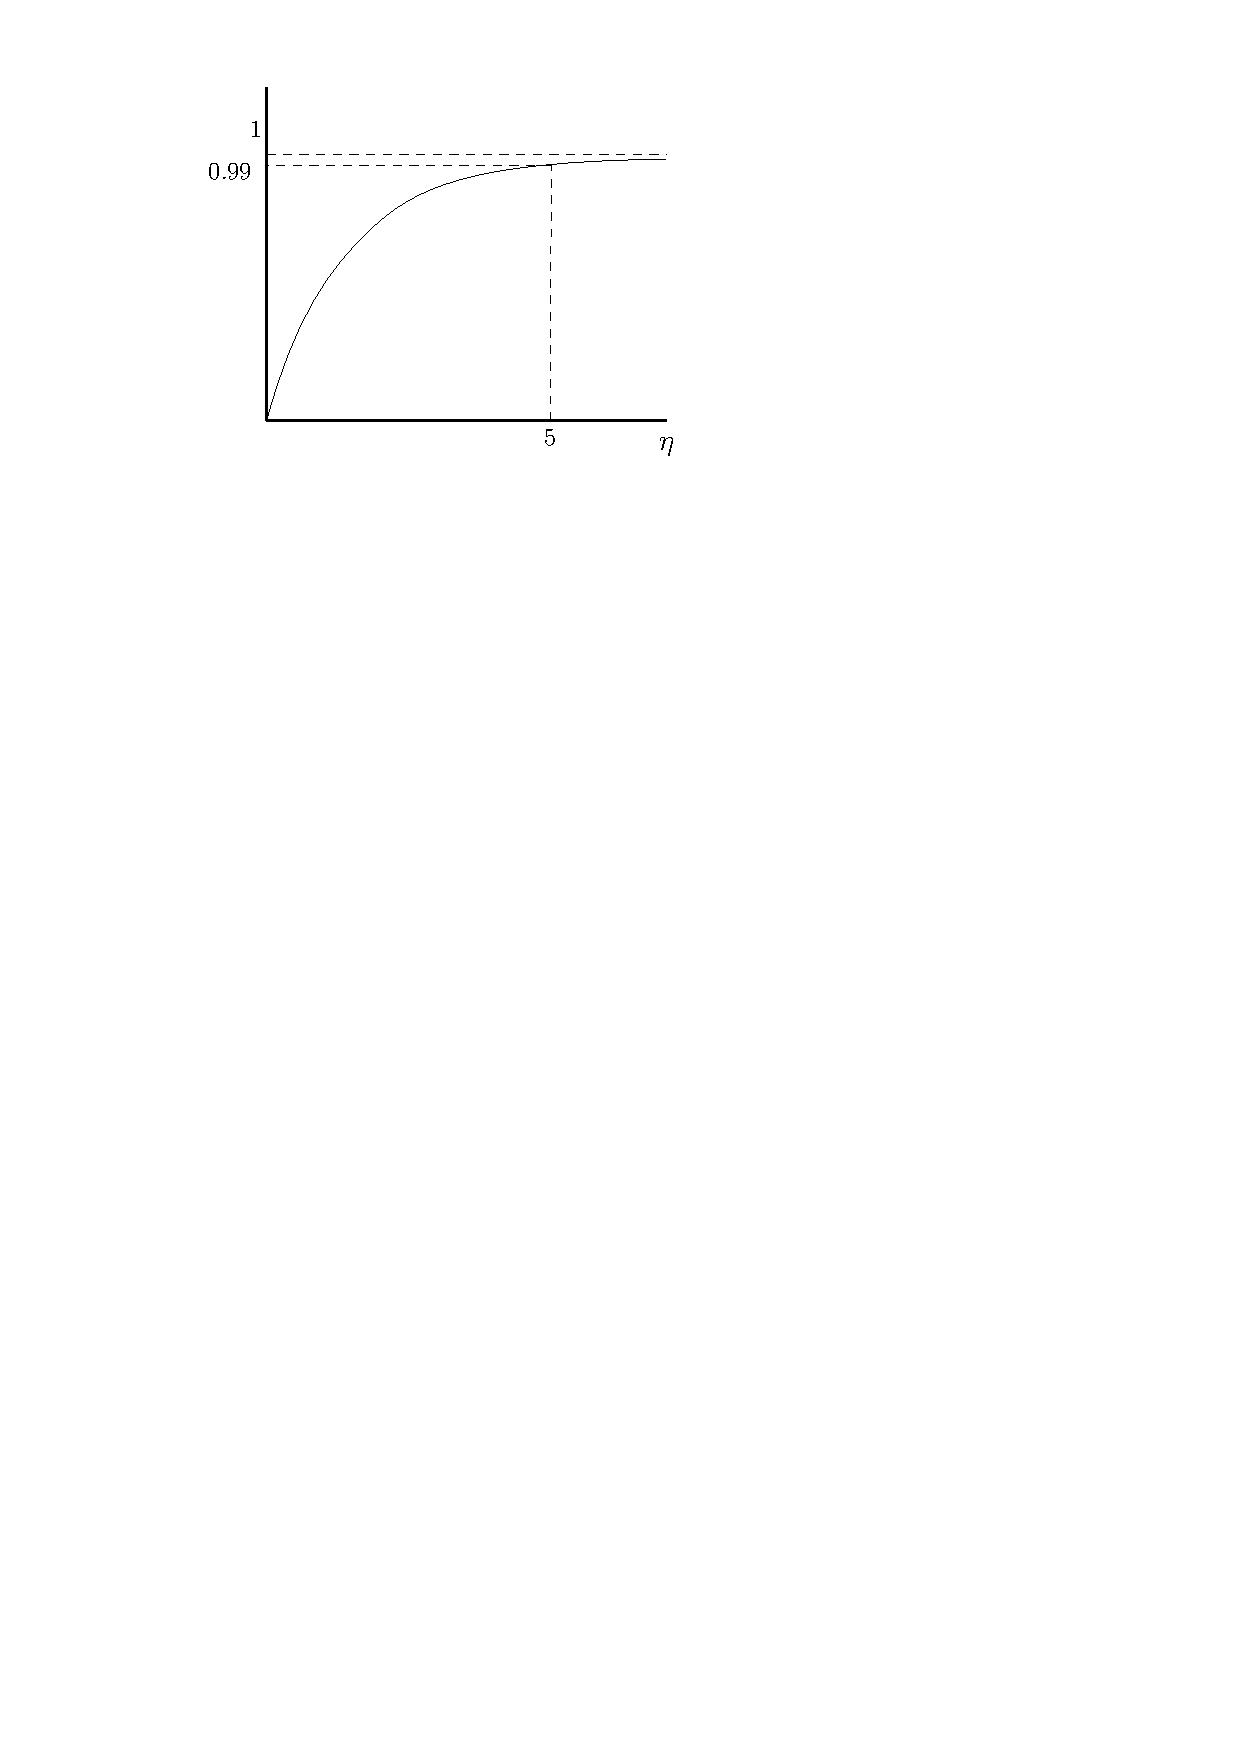
\includegraphics[scale=0.8]{./7.4 Strato limite/7.4-5}
		\centering
		\caption{99\% della velocità esterna}
	\end{figure}
%
Si vede che in quel punto $\eta = 5$, si può risalire allo spessore:
%
	\begin{equation*}
		\begin{gathered}
		\eta = 5 = \frac{Y}{x^{1/2}} = \frac{y}{\epsilon x^{1/2}} = \frac{y^d}{ {\left( \frac{\nu}{L_r U_r} \right)}^{1/2} {\left( \frac{x^d}{L_r} \right)}^{1/2}  } = \frac{y^d}{\nu^{1/2} U_r^{-1/2} {x^d}^{1/2} }\\
		\text{Si definisce}\\
		\delta_{0.99} = y^d_{\eta = 5} = 5 \nu^{1/2} U_r^{-1/2} {x^d}^{1/2} = 5 x^d R_{ex}^{-1/2}
		\end{gathered}
	\end{equation*}
%
È lo spessore dello strato limite, il grafico va come una radice quadrata ed è l'inverso del grafico dello sforzo: 
%
	\begin{figure}[ht]
		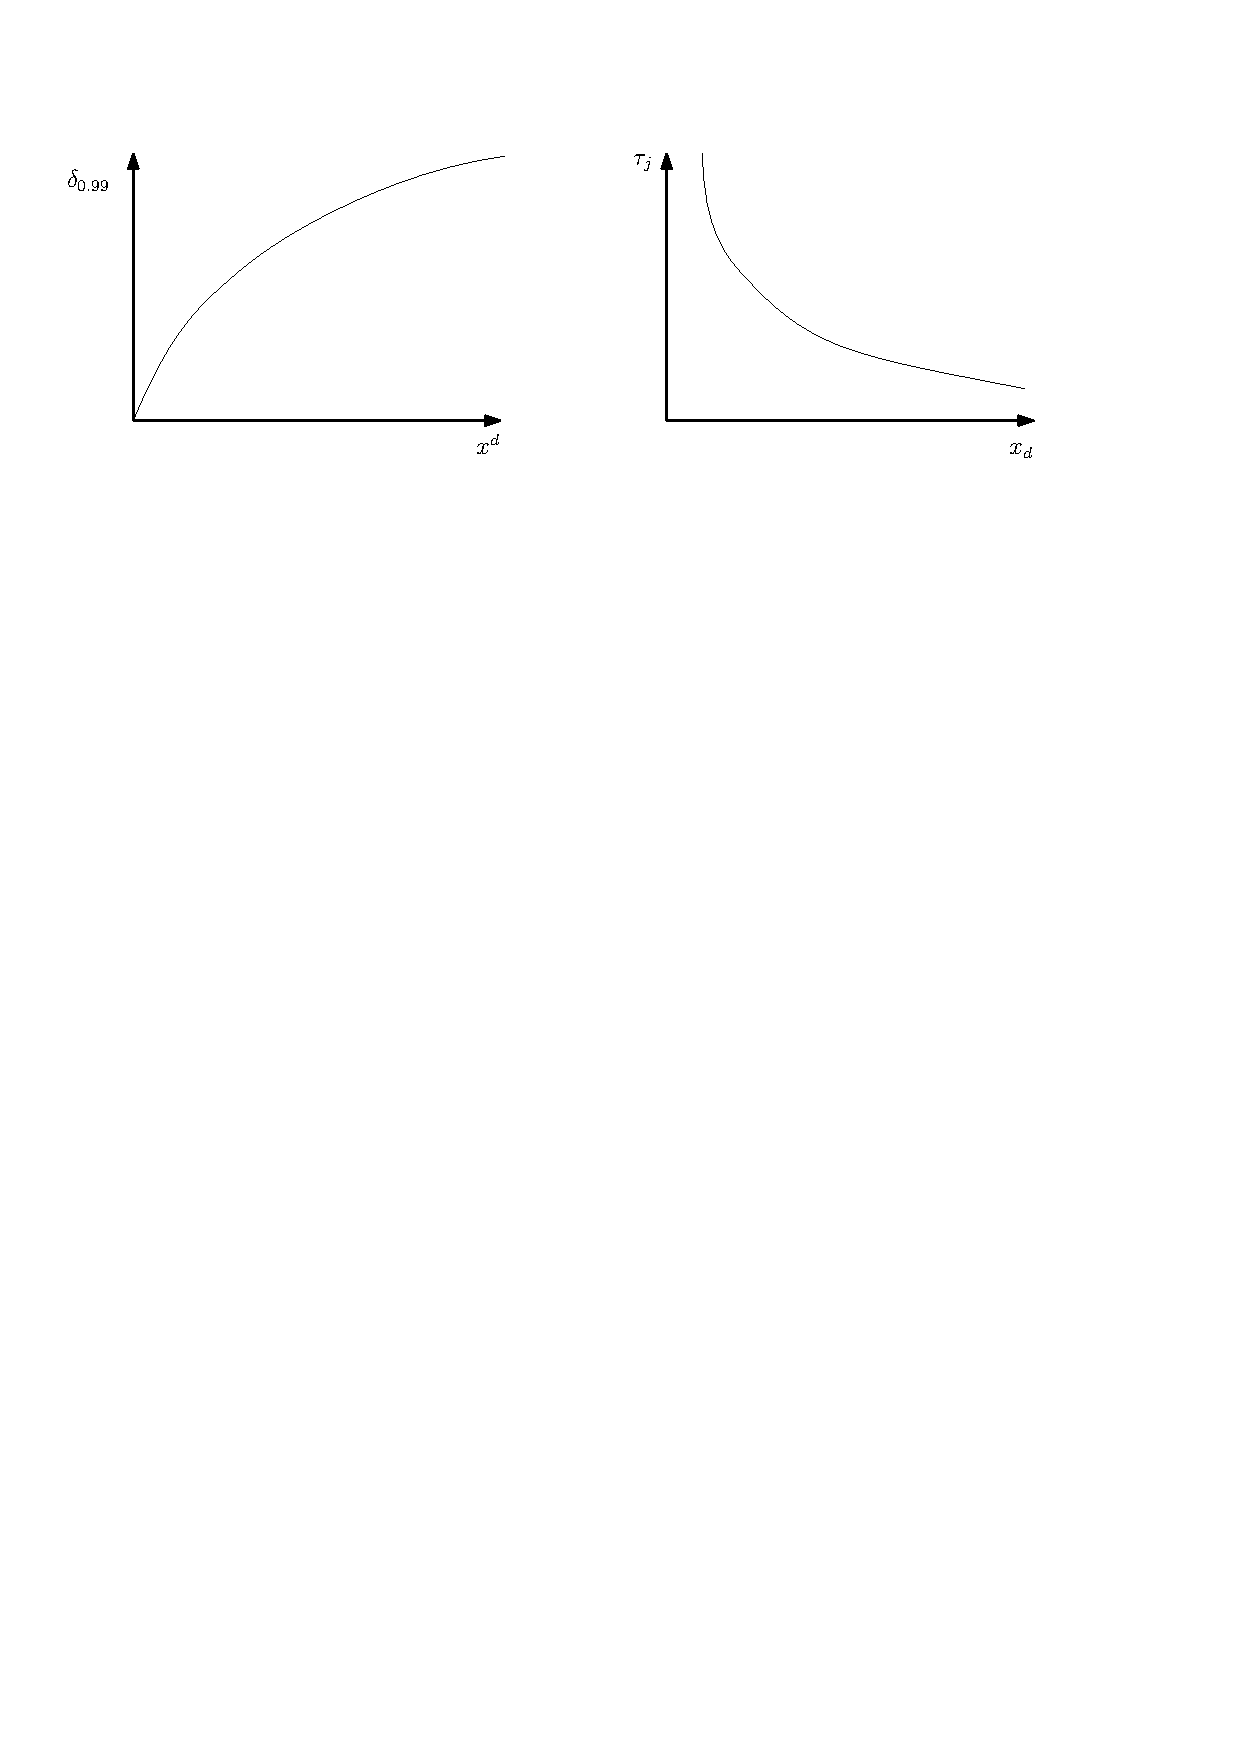
\includegraphics[scale=0.7]{./7.4 Strato limite/7.4-6}
		\centering
		\caption{Sforzo e strato limite}
	\end{figure}
%

Ci sono anche altri modi di definire lo spessore, ad esempio lo spessore di spostamento.
Se si avesse una $u$ costante il suo integrale (cioè la portata) sarebbe differente da quello del profilo reale.
Vedendolo su un grafico, è come se questa differenza si potesse compensare spostando la parete di una quantità $\delta_*$, che è uno spessore tale che la portata calcolata come se valessero le equazioni di Eulero sia uguale alla portata reale:
 %
	\begin{figure}[ht]
		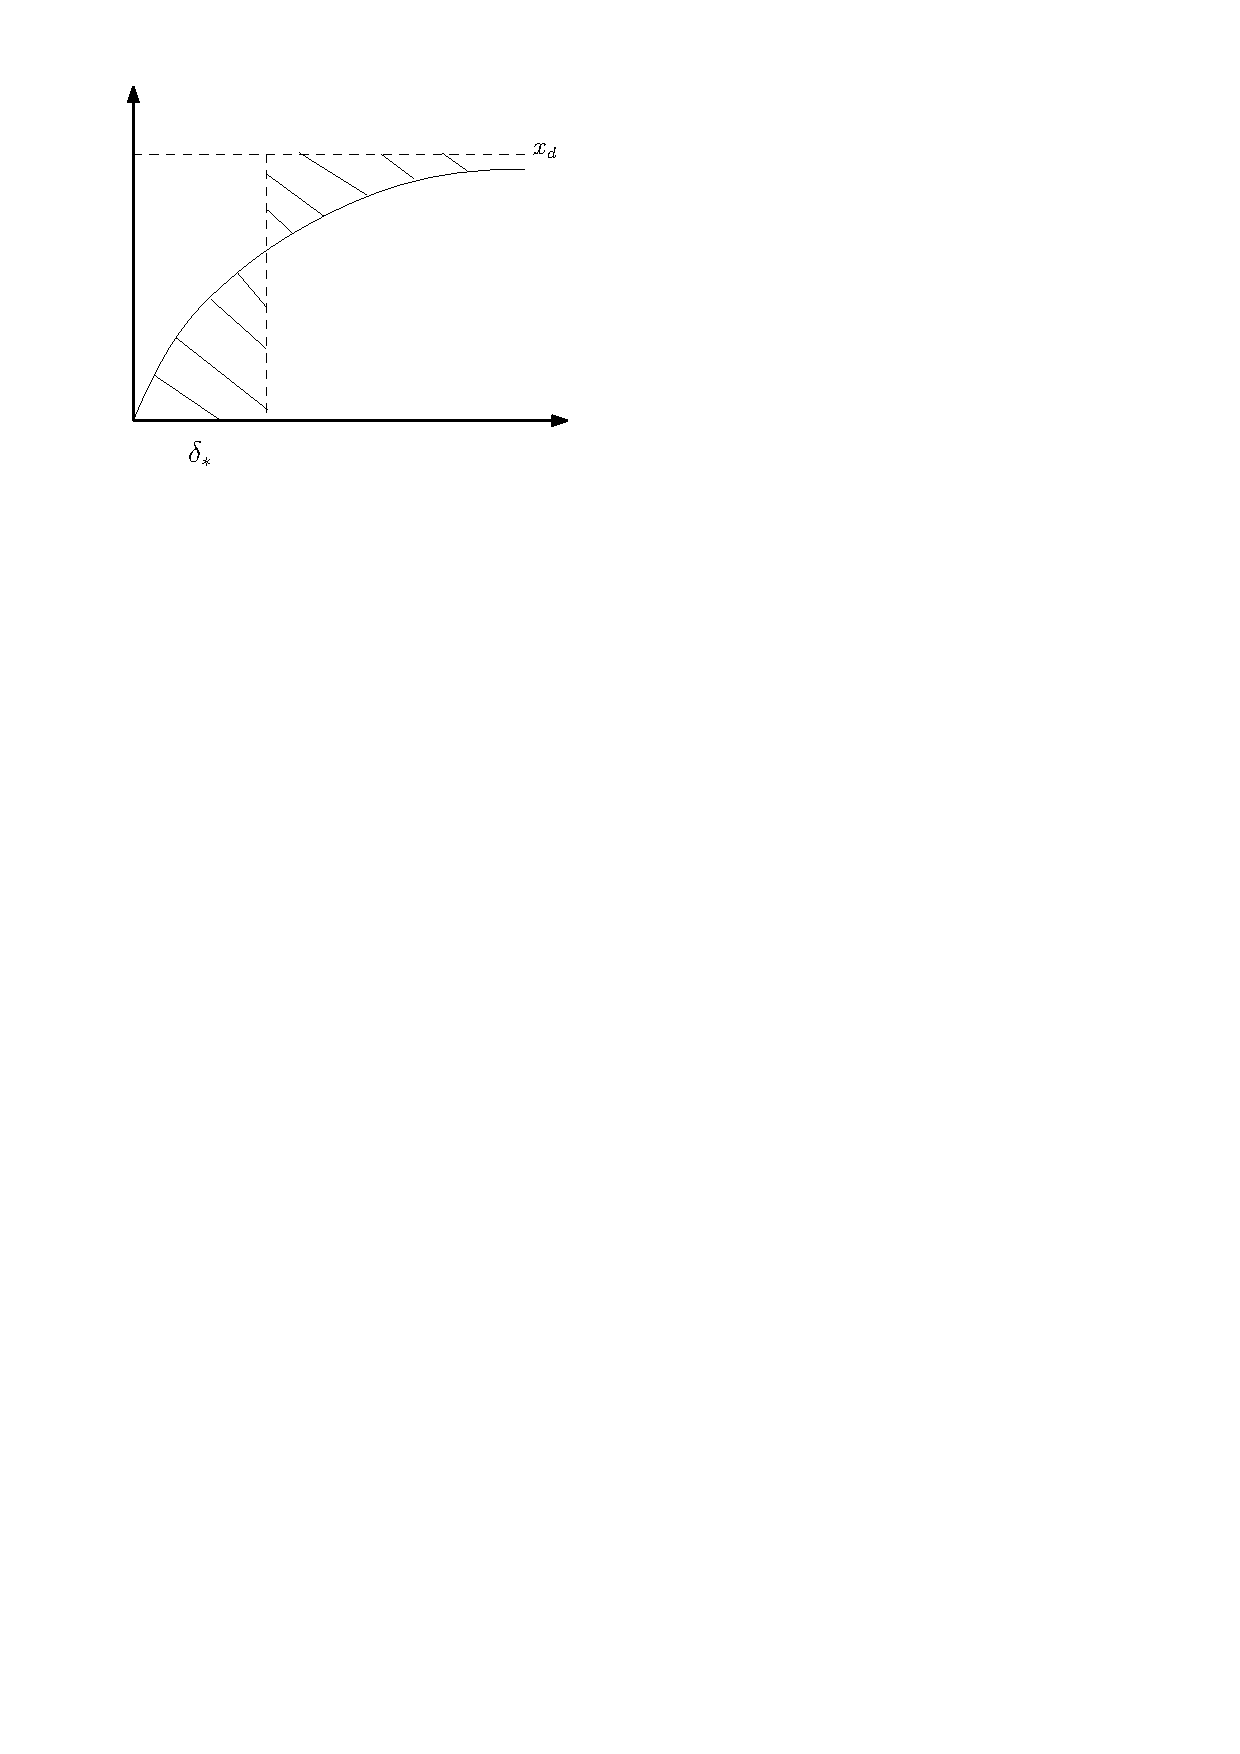
\includegraphics[scale=0.7]{./7.4 Strato limite/7.4-7}
		\centering
		\caption{Spessore di spostamento}
	\end{figure}
%
Da questo è possibile trovare il valore di $\eta$ corrispondente:
 %
	\begin{figure}[ht]
		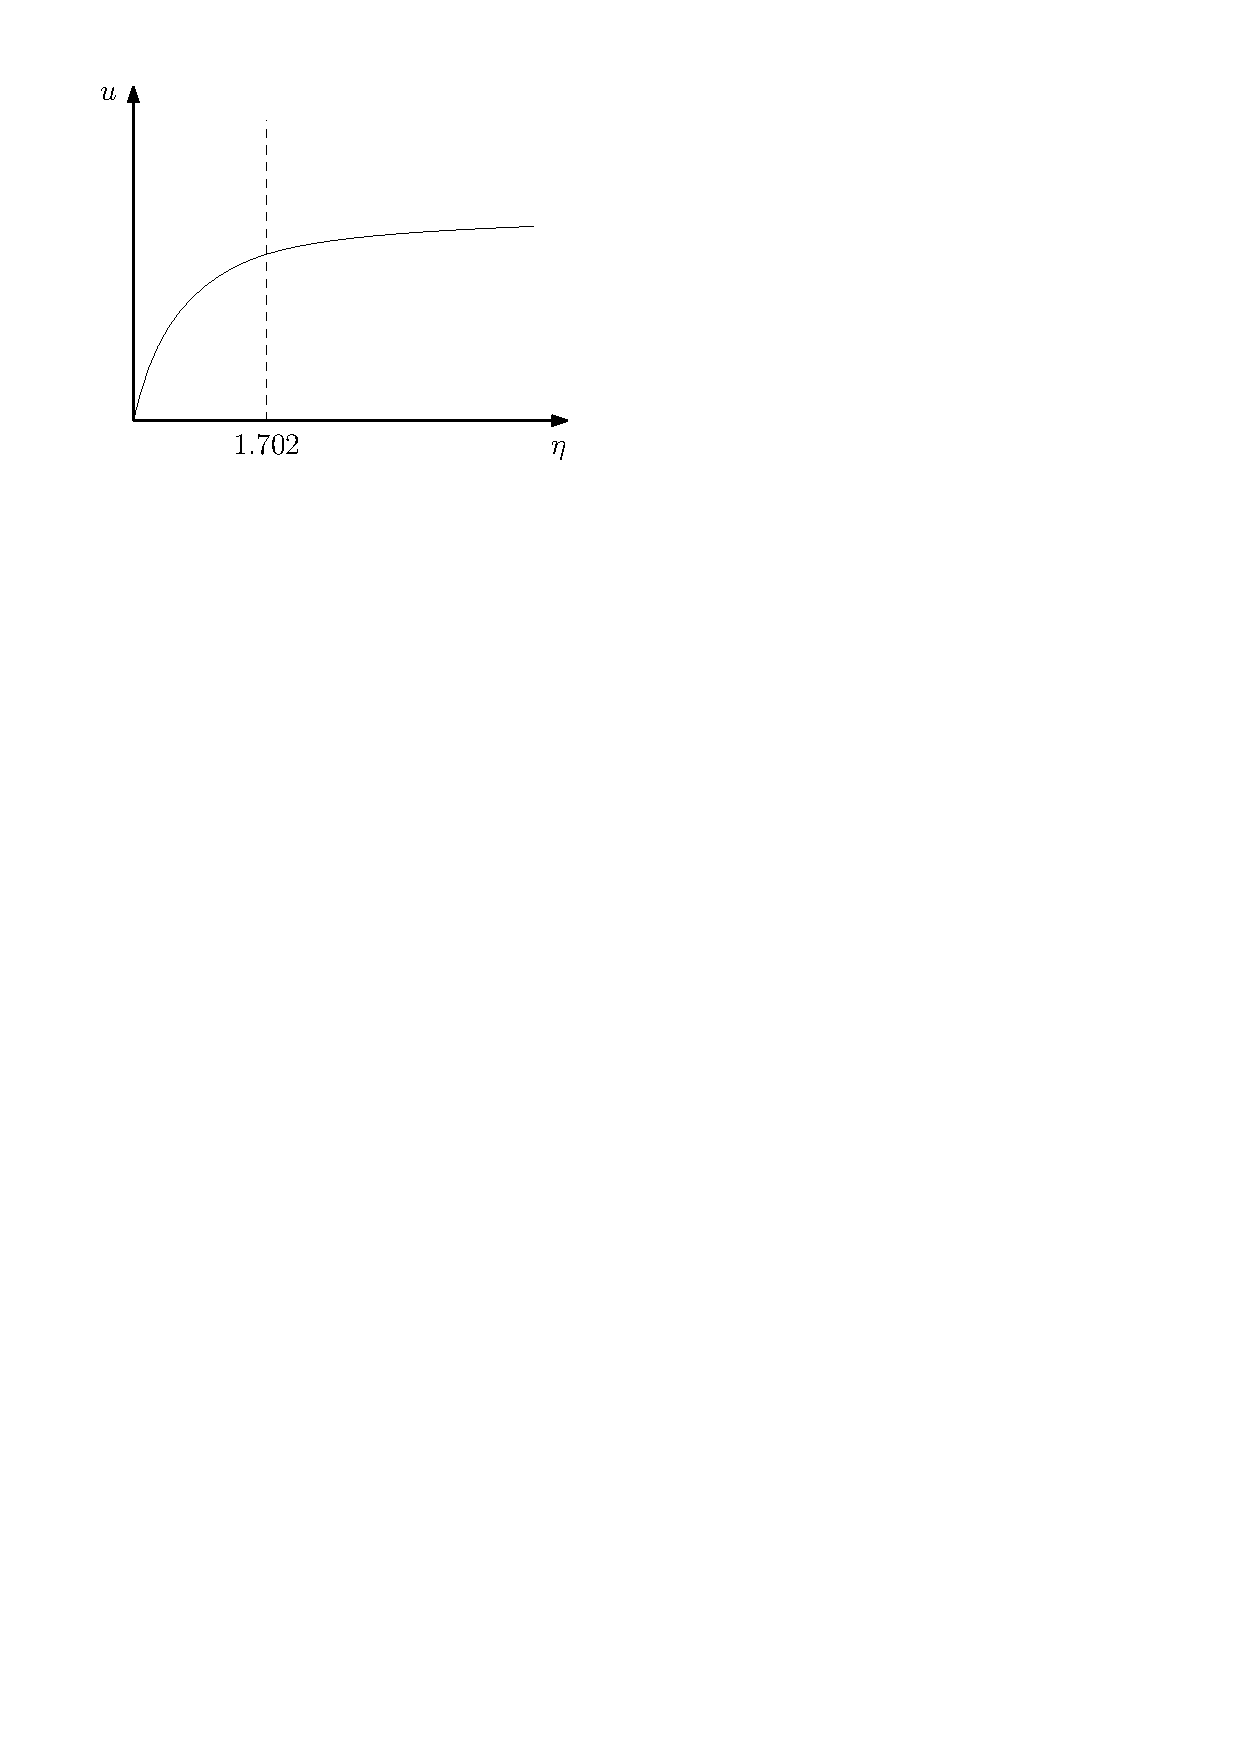
\includegraphics[scale=0.8]{./7.4 Strato limite/7.4-8}
		\centering
		\caption{Valore di $\eta$}
	\end{figure}
%
Quindi si trova che lo spessore di spostamento è:
%
	\begin{equation*}
		\delta_* = 1.702 \nu^{1/2} U_r^{-1/2} {x^d}^{-1/2}	
	\end{equation*}
%	

Altra definizione è quella dello spostamento di quantità di moto:
%
	\begin{equation*}
		\theta = 2.5 \nu^{1/2} U_r^{-1/2} {x^d}^{1/2}
	\end{equation*}
%

%SUBSECTION
\subsection{Imbocco di un tubo}
All'imbocco di un tubo inizialmente si hanno due strati limite distinti, che possono essere studiati separatamente.
Ad un certo punto questi si incontreranno, il problema non sarà più quello di due strati limite ma quello dell'imbocco di un tubo.
Ad un certo punto il flusso nella tubazione diventerà quello di Poiseuille, all'inizio era quello di Eulero, quindi in mezzo si avrà una situazione intermedia:
 %
	\begin{figure}[ht]
		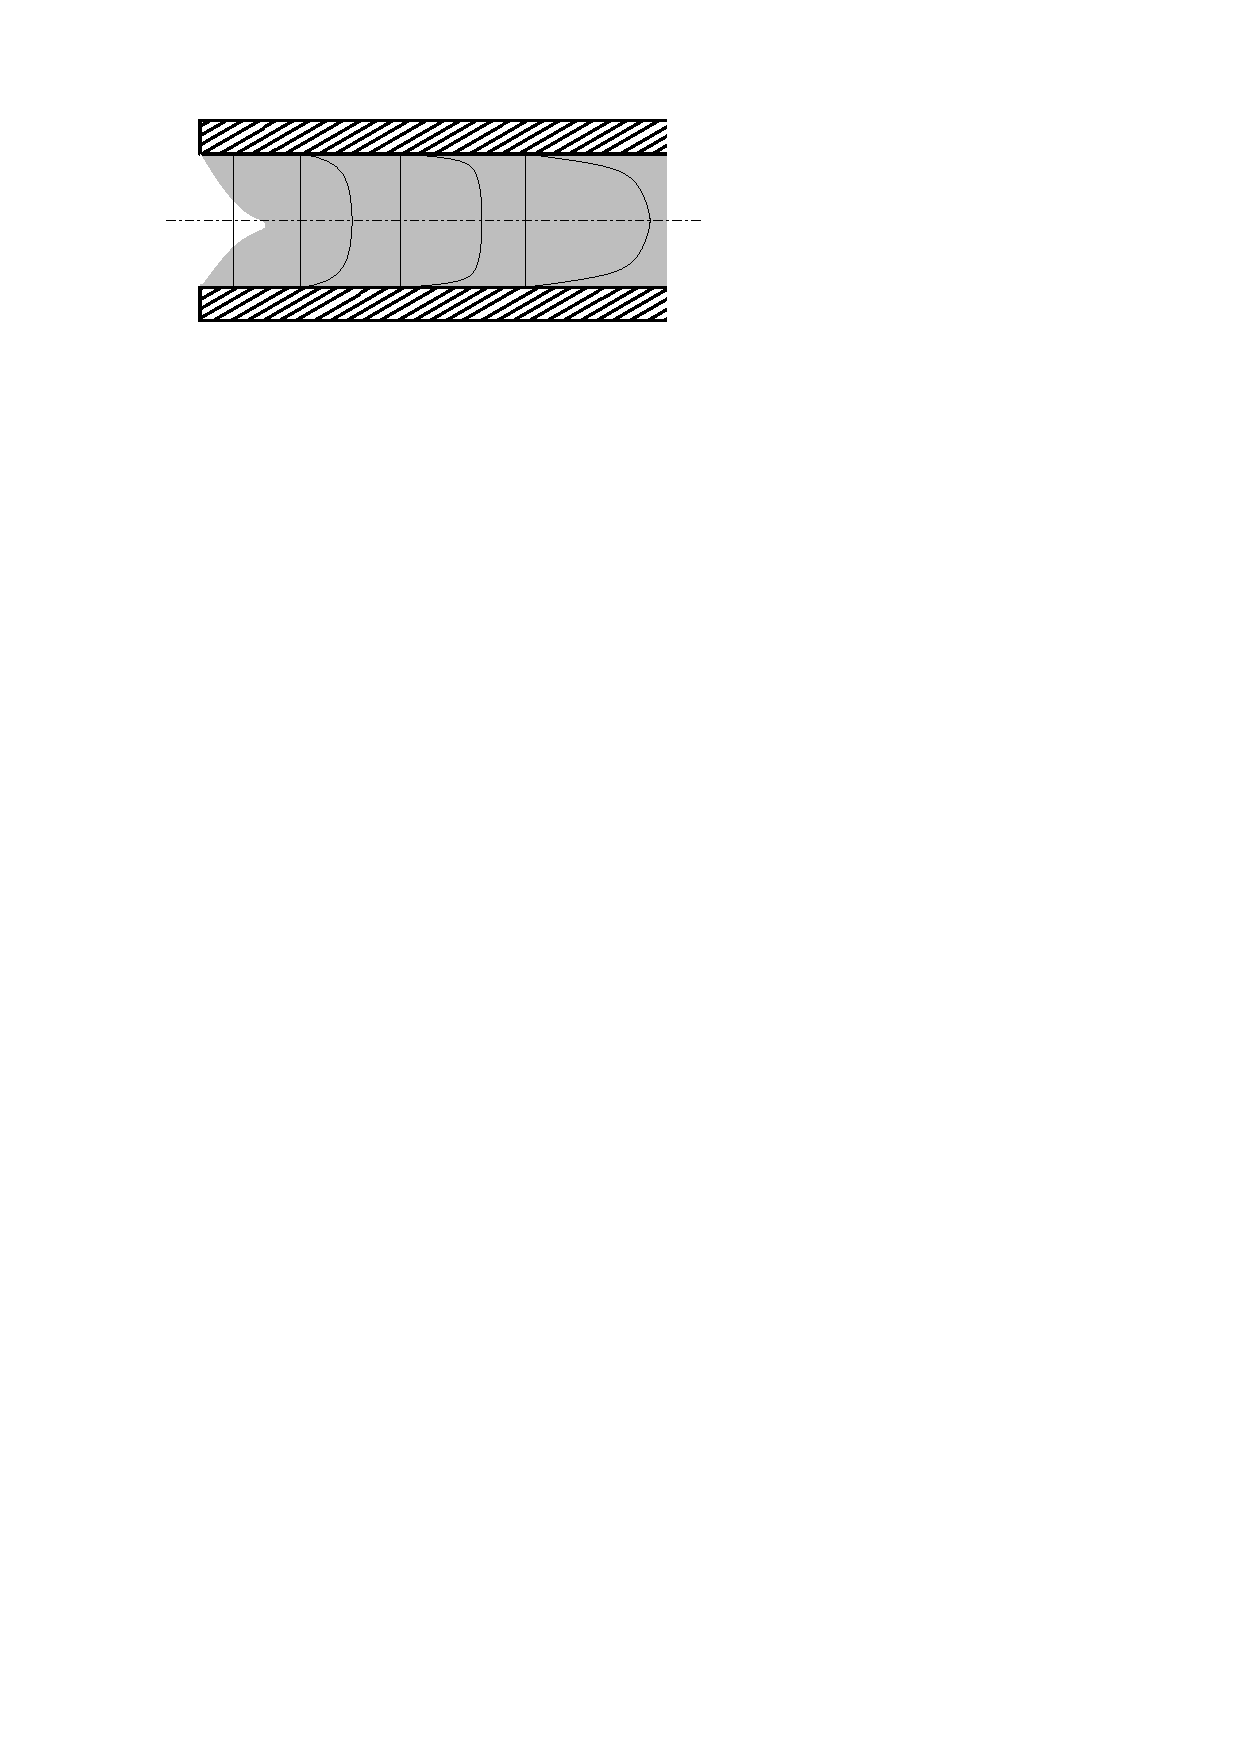
\includegraphics[scale=1.0]{./7.4 Strato limite/7.4-9}
		\centering
		\caption{Imbocco di un tubo}
	\end{figure}
%


\subsection*{Bibliografia 7.4}
\cite[Cap.\ 10.5]{CengelCimbala}\\
\cite[Cap.\ 11.1, 11.2]{PnueliGutfinger}